\documentclass[11pt]{report}

\usepackage{epsf,amsmath,amsfonts}
\usepackage{graphicx}
\usepackage{listings}
\usepackage{hyperref}
\usepackage{placeins}

\begin{document}

\title{MPAS Developers Guide}
\author{MPAS Development Team}

\maketitle
\tableofcontents

%-----------------------------------------------------------------------

\chapter{Summary}
This document is intended to describe general development practices within the
MPAS project. The information contained should be read prior to starting a
project within the MPAS framework. Instructions can be used by MPAS core
developers, or external developers. Notes specific to external developers are
made where relevant.

\section{Becoming a MPAS Developer}
The preferred approach to contributing source code to the MPAS-Dev repositories
is via a fork of the release repository. If the preferred approach is not
workable, developer access to the MPAS-Dev GitHub project needs to be approved
by core maintainers. Prospective developers should send the following
information to the relevant core maintainers.
\begin{itemize}
	\item What is your GitHub user name? \\
		(can be acquired at \href{http://www.github.com}{github})
	\item Can your work be completed in a fork of the release repository?
	\item If no, please explain the reason.
	\item What core do you intend to develop?
	\item What work do you intend to contribute to MPAS?
\end{itemize}

\chapter{Repository Descriptions}
The MPAS project contains several repositories. Some of the repositories are
private for development efforts while some are public for users and releases.
These repositories are described below.

\section{Main Development/Release}
The main MPAS repositories are described in this section. Users interested in
implementing a new feature only need to interest themselves in section
\ref{subsec:mpas_release}.


\subsection{MPAS -- Private Repository}
This main MPAS development repository is located
\href{https://github.com/MPAS-Dev/MPAS}{here}.  This repository will be where
the majority of MPAS development occurs.  Instructions on using it to add a
feature are below in section \ref{sec:forks}. This is a private repository for
development efforts.

\subsection{MPAS-Legacy -- Private Repository}
The MPAS-Legacy repository is located
\href{https://github.com/MPAS-Dev/MPAS-Legacy}{here}. It provides a linear
history of the previous SVN repository's trunk/mpas directory. It is provided
only for debugging purposes and no development should/will be carried out using
it.

\subsection{MPAS-Release -- Public Repository}
\label{subsec:mpas_release}
The main MPAS release repository is located
\href{https://github.com/MPAS-Dev/MPAS-Release}{here}.  Users should refer to
this repository for bug fixes, issues, and major releases for MPAS.

Users who wish to implement a new feature, and have that feature merged into
the MPAS repository should follow the instructions on code requirements and
repository layout as an MPAS developer would. Forks should be made of this
release repository for this type of development rather than the MPAS developer
repository. New features will have to undergo a code review before any merge
onto the release repository.

\subsection{Layouts}
The MPAS, MPAS-Release, and MPAS-Legacy repositories are all laid out as follows.
\begin{lstlisting}
MPAS
|-Makefile
\-src
  |-driver
  |-registry
  |-framework
  |-operators
  |-external
  |-inc
  |-core_*
  \-Makefile
\end{lstlisting}

Although there are more files/directories than are listed these are the
relevant directories for source code modifications.

The src directory contains all source code related to MPAS, whether it is shared
or not.

Shared parts of MPAS belong in either the driver, external, framework,
operators, or registry directories.

registry contains the parsing code for Registry. Registry is used for easy
modification of variables within a specific MPAS core. Each core has it's own
Registry.xml file which defines a list of dimensions, namelist options,
variables, and other information specific to that core. On compile time, the
registry parser ({\it parse}) is built. This parser then parses the Registry.xml file
and generates some Fortran code, which is stored in src/inc. It is then
included at various places within framework to define all of the necessary
things. The code generated from registry defines the domain structure for a
core, and routines associated with building domain. Domain will be discussed in
section \ref{sec:code_intro}.

driver contains general code for building the MPAS executable, and the general
structure of how an MPAS executable looks.

external contains external code to MPAS that is used within MPAS, i.e. ESMF
time keeping routines.

framework contains shared code related to the framework of MPAS. This includes
the I/O layer, communication routines, and definitions of the data types.

operators contains shared code used for computing specific quantities on an
MPAS grid. This includes radial basis function interpolation.

inc is an empty staging directory that registry fills at compile time.

Non-shared parts of MPAS belong under the remaining directories. As an example,
the core\_sw directory represents the shallow water dynamic core within the
MPAS framework. Other directories named core\_ are either dynamical cores, or
parts of other dynamical cores.

Most developers will only work under their specific core directory, and should
not modify code in another core without permission.

\section{MPAS-Testing -- Private Repository}
The MPAS-Testing repository is located 
\href{https://github.com/MPAS-Dev/MPAS-Testing}{here}. This repository will
contain software to setup and run MPAS test cases.

\subsection{Layout}
The MPAS-Testing repository is laid out as follows:
\begin{lstlisting}
MPAS-Testing
|--sw (Test Cases for Shallow water core)
|--ocean (Test Cases for Ocean core)
|--atmosphere (Test Cases for Non-Hydrostatic Atmospheric core)
\--shared (Test Cases for shared parts of MPAS)
\end{lstlisting}

\section{MPAS-Documents -- Private Repository}
The MPAS-Documents repository is located
\href{https://github.com/MPAS-Dev/MPAS-Documents}{here}. This repository will
contain all MPAS related documents. This includes design documents, users
guides, developers guides, etc.

\subsection{Layout}
The MPAS-Documents repository is laid out as follows:
\begin{lstlisting}
MPAS-Documents
|--design_documents
|  |--shared (Design documents for project in shared directory)
|  |--sw (Design documents for shallow water core)
|  |--ocean (Design documents for ocean core)
|  |--atmosphere (Design documents for Non-hydrostatic atmosphere core)
|--users_guide
|  |--shared (Shared parts of users guide)
|  |--sw (Shallow water specific parts of users guide)
|  |--ocean (Ocean specific parts of users guide)
|  |--atmosphere (Non-hydrostatic Atmosphere specific parts of users guide)
\--developers_guide (This document)
\end{lstlisting}

\section{MPAS-Tools -- Private Repository}
The MPAS-Tools repository is located
\href{https://github.com/MPAS-Dev/MPAS-Tools}{here}. This repository will
contain all MPAS related tools.

\subsection{Layout}
The layout of the MPAS-Tools repository is as follows:
\begin{lstlisting}
MPAS-Tools
|--analysis (All tools related to analysis)
|--grid_gen (All tools related to grid generation)
|--python_scripts (All general purpose python scripts)
\--visualization (All visualization tools)
\end{lstlisting}

To promote reuse of previously developed tools, tools won't be stored in core
specific directories. This way, a developer is encouraged to browse other tools
and see if a feature is implemented elsewhere.

\section{MPAS-Data -- Public Repository} 
The MPAS-Data repository is located \href{https://github.com/MPAS-Dev/MPAS-Data}{here}. This repository
will contain data required to run specific MPAS models. This data does not
include input files related to specific runs, it is intended to house general
data that doesn't change between runs.

\subsection{Layout}
The layout of the MPAS-Data repository is as follows:
\begin{lstlisting}
MPAS-Data
|--framework (Data required for parts of framework)
|--operators (Data required for parts of operators)
\--core_* (Data required for specific cores)
\end{lstlisting}

\chapter{Development}
The repositories are all hosted on github. The typical life-cycle of a project is as follows:
\begin{enumerate}
	\item Create a design document for the project. \\
		  (e.g. section \ref{sec:design_documents})
	\item Visit appropriate repository website. \\
		  (e.g. \href{https://github.com/MPAS-Dev/MPAS-Release}{Release Repository})
	\item Create a fork of the repository. \\
		  (e.g. section \ref{sec:forks})
	\item Locally clone the newly created fork. \\
		  (e.g. git clone https://fork/url)
	\item Create a branch within the fork, for the new feature or bug fix. \\
		  See section  \ref{sec:branches} for a description of our branching strategy. \\
		  (e.g. git checkout -b new\_branch)
	\item Develop branch. \\
		  (e.g. touch src/framework/work\_complete.F \&\& git commit -a)
	\item Push complete branch to remote fork. \\
		  (e.g. git push -u origin new\_branch)
	\item Submit a pull request to merge branch on fork to main repository master. \\
		  (e.g. section \ref{sec:pull_request})
\end{enumerate}

Projects don't have to follow this example verbatim, but this at least
gives a general overview of the process. Some details related to this
life-cycle will be described in the following sections.

Code level requirements are described in chapter \ref{chap:code-guidelines}.

\section{Design Documents}
\label{sec:design_documents}
Design documents are recommended for projects that contribute significant
changes to either a core or to MPAS in general. They should clearly describe
the justification for the project, and the changes and impacts of the project.
Core maintainers reserve the right to deny a pull request that lacks a design
document.

Developers can refer to
\href{http://mpas-dev.github.com/files/documents/mpas\_ddt\_redesign.pdf}{DDT
Redesign} and
\href{http://mpas-dev.github.com/files/documents/implicit\_vert\_diff\_design.pdf}{Implicit
Vertical Mixing (MPAS-Ocean)} for examples of design documents that have been
previously completed.

\section{Forks}
\label{sec:forks}
A fork is a user specific copy of another repository. Forks can only be made
from repositories a user has pull access to. Permissions on a fork remain the
same as the original repository (e.g. pull teams still have pull access over
the fork), with the exception that the user creating the fork gains elevated
admin permissions over the newly created fork.

A fork can be thought of exactly like a branch. Except it lives in a separate
repository, and contains it's own private history. As forks remember where they
came from, they can still be merged onto the repository they were created from.

The \href{https://help.github.com/articles/fork-a-repo}{github fork guide} can
be used to learn how to create a fork of a repository.

The user who created a fork can easily delete the fork, without fear of
destroying the original repository.

\section{Pull Requests}
\label{sec:pull_request}
A pull request represents several things in our development process. At it's
basis, a pull request is a merge request. It describes a branch that a
developer wishes to have merged onto some alternate branch or repository. In
addition to a request for a merge, it fully describes the changes involved in
the merge, along with allowing for a full review of the merge prior to the
actual merge.

Other developers can review and comment on pull requests. A pull request will
be assigned to the relevant core maintainer.

Github provides guides for
\href{https://help.github.com/articles/creating-a-pull-request}{creating a pull
request}, \href{https://help.github.com/articles/using-pull-requests}{using a
pull request}, and
\href{https://help.github.com/articles/merging-a-pull-request}{merging a pull
request}. Please refer
to these guides for more instructions on pull requests.

\section{Branch Strategy}
\label{sec:branches}
As a developer, most work will be completed in a branch. This branch can be one
of several types of branches. To give an overview of the current branching
strategy, please see
\href{http://nvie.com/posts/a-successful-git-branching-model/}{this document}. 

The name of a branch should be descriptive and tell where the feature addition
will be. For example, if the branch is intended to implement multiple blocks,
the majority of its work would take place in framework. A good name for the
branch would then be framework/multiple\_blocks.

Feature branches should only be created from the develop branch. This allows a
cleaner work flow when planning releases. Any features that have been merged
onto develop can be staged for release. This means, if you submit a pull
request for a feature to be merged onto the MPAS-Dev version of develop, you
are giving consent for it to be included in the next coordinated release.

\section{Release Branches}
\label{sec:release-branches}
One of the various branch types that developers will see in the shared
repository is a release branch. This release branch is used to prepare the code
for a new release, and comes with some guidelines of use.

As per the branch document listed in section \ref{sec:branches}, release
branches should branch off of develop. Once they are complete, they are merged
into both develop and master. After they are merged into master, that commit is
tagged with a new version number, and then pushed into the MPAS-Release
repository for a public release.

A release branch can be thought of as a feature freeze. Once the release branch
is created, no new features can make it into the next release. The only commits
that can be appended to a release branch are clean up and bug fix commits.

Due to the requirement that anything merged into develop can be released at any
point in time, a group of developers can decide they want to begin the release
process at any point in time. The guidelines for the release process are as
follows, however the flexibility of these guidelines is at the discretion of
the group performing the release.
\begin{itemize}
	\item From any point in time, the soonest date that can be targeted for release is 1 month from the current date.
	\item Once a release date is selected, it should be anounced to the MPAS developers list to alert all core developers.
	\item There is a minimum lag time of 2 weeks between the announcement of a release date, and the creation of a release branch. This is to allow developers to finish any projects that are close to being complete, that they would like to be part of the next release.
	\item After the 2 weeks are up, a release branch can be created from the tip of the develop branch.
	\item The first commit to a release branch should be updating the version numbers.
	\item The maximum time a release branch is allowed to exist is 2 weeks. After the release branch has been in existence for 2 weeks, it is assumed all core maintainer groups are finished with any efforts to prepare for release. At this point, the release branch is complete.
	\item The release branch is then merged into master and develop.
	\item The commit on master is tagged with the new version number.
	\item The master branch is then pushed to the MPAS-Release repository.
\end{itemize}

These guidelines lay out a minimum amount of time a release cycle should
consume. However, the core group that intends to release should announce the
targeted date of release as soon as they have one selected.

The creation of a release branch can be delayed. A request for the delay of
creation should be made through the mpas-developers mailing list. Any other
core is allowed to deny the request for any reason. It should also be
understood that delaying the creation of the release branch does not delay the
actual release itself.

\section{Version Numbers}
\label{sec:version-numbers}
MPAS will have a two number versioning system. For example, 0.0 or 1.5. In this
case, the first digit refers to coordinated release. The second digit refers to
intermediate bug fixes.

Referring to the branching strategy in section \ref{sec:branches}, coordinated
releases occur when a release branch is created off of develop and merged back
into develop and master. While an intermediate bug fix happens when a branch is
created off of master and merged back into master and develop.

The minor version (second digit) of MPAS increments when a bug fix branch is
merged into master. These merges never include feature additions to any of the
cores or shared framework.

The major version (first digit) of MPAS increments when a release branch is
merged into master. A release branch includes {\bf all} of the features that
were present on the develop branch when it was created. The release branch
persists for some period of time to allow core developers to "clean up" any
issues they have prior to release. After the grace period, the release branch
is merged into master and develop and the major version of MPAS increments by
1, while the minor version is reset to 0.

\chapter{Development guidelines}
\label{chap:code-guidelines}
As developers of MPAS, we attempt to make the code look as uniform as we can
across the entire code-base. In order to enforce this, there are a set of
guidelines developers should follow.

\begin{itemize}
	\item Each core has a name, and an abbreviation. For example, the shallow water core is called sw and it's abbreviation is sw, but the ocean core is called ocean and it's abbreviation is ocn.
	\item All subroutines should be named in a manner which prevents namespace conflicts. \\ 
		  Shared functions/subroutines are simply named mpas\_subroutine\_name.\\ 
		  Core specific functions/subroutines are named mpas\_abbrev\_subroutine\_name (where abbrev is replaced with the cores abbreviation). \\
		  e.g. mpas\_atm\_time\_integration
    \item Subroutine names should all be lower case, with underscores in place of spaces (e.g. see above).
	\item Variable names should be mixed case (e.g. cellsOnCell rather than cells\_on\_cell).
	\item In general, variable names should be self-descriptive (e.g. nCells rather than n).
	\item Subroutines and modules should be appropriately documented. Shared portions of MPAS code use doxygen comments, but core developers are free to decide what method of documenting they prefer.
	\item Development of shared parts of MPAS need reviews from multiple core maintainers prior to a merge.
	\item Development within a core should be approved by other core developers before being merged into that core.
	\item Development within a core should follow the practices of that core's developer group, for documentation etc.
	\item Core related testing is the responsibility of that core's maintainers/developers.
%	\item ....more guidelines?
\end{itemize}

Core maintainers need to approve changes before the changes appear on the
shared repository. Core maintainers are also responsible for reviewing changes
to shared code that affect multiple cores.

\section{General Code Introduction}
\label{sec:code_intro}
The MPAS framework makes extensive use of derived data types. A lot of these
derived data types are defined in src/framework/mpas\_grid\_types.F, but some
of the data types are not defined until build time. Registry is used to define
both fields and structures. A field is the lowest level of data with in the
MPAS framework, and contains a description of the field along with the actual
field data. The field types that are allowed are defined in the previously
mentioned file, and Registry makes use of these type definitions.

A structure is a larger grouping of fields, and dimensions. Structures can have
multiple time levels, or a single time level. A structure can be used to group
fields and define a part of the model, e.g. the mesh definition.

Structures are grouped into blocks. A block can be thought of as all relevant
information for a particular part of your domain. The entire domain is
subdivided horizontally into blocks. Within the model, blocks are stored in a
linked list.

The largest structure is the domain, which defines all blocks that are part of
a particular MPI processes computational domain. 

The following diagram is provided as a visual aid for the layout of data within
the MPAS framework. It is not exhaustive, so please refer to any core specific
references to get a more complete list of how derived data types are laid out
in the specific core.

\begin{figure}[htp!]
	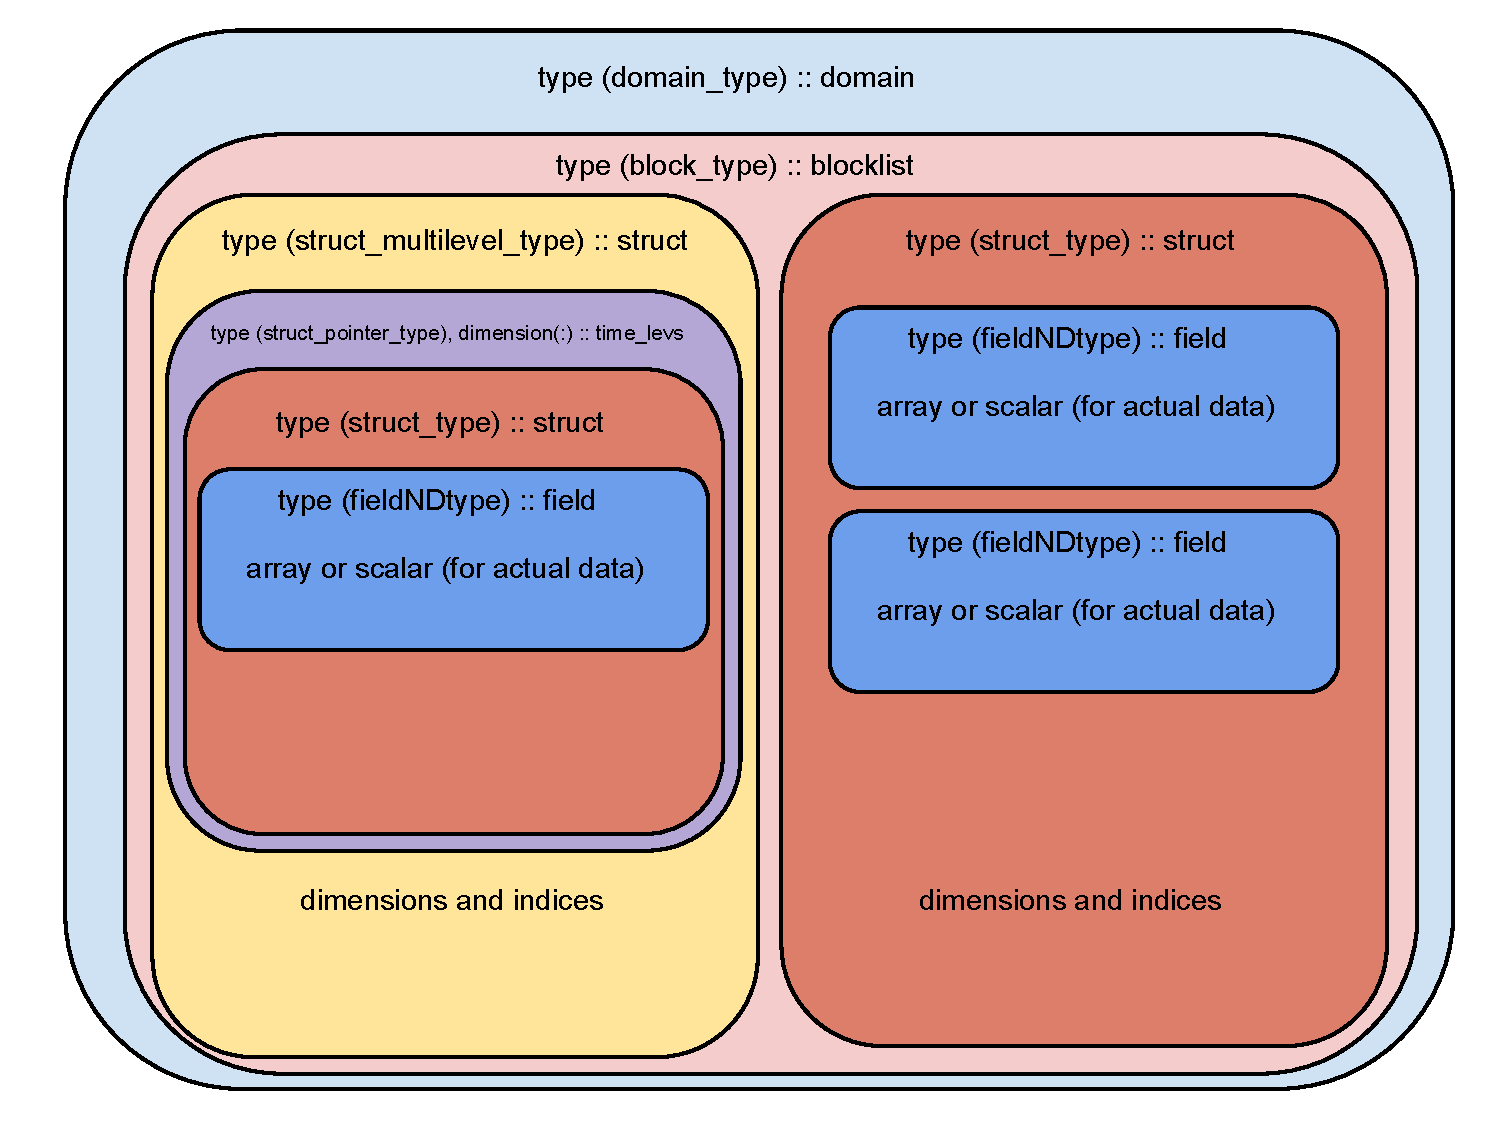
\includegraphics[scale=0.5]{figures/ddt_diagram.pdf}
	\caption{Visual diagram of MPAS derived data type layout.}
	\label{fig:ddt_diagram}
\end{figure}
\FloatBarrier


In the actual MPAS code, this diagram converts to the following lines.
{\tiny
\begin{lstlisting}
domain % blocklist % struct1 % field1 % array
domain % blocklist % struct1 % field2 % scalar

domain % blocklist % struct2 % time_levs(1) % struct2 % field1 % array
domain % blocklist % struct2 % time_levs(1) % struct2 % field2 % scalar
\end{lstlisting}
}

As the blocklist structure is a linked list of blocks, one can iterate over the
list of blocks in the following manner.

\begin{lstlisting}[language=fortran,escapechar=@,frame=single]
type (block_type), pointer :: block_ptr

block_ptr => domain % blocklist
do (while(associated(block_ptr))
	... do stuff on block ...
	block_ptr => block_ptr % next
end do
\end{lstlisting}

\section{Addition of New Variables}
In order to create new fields or structures, a developer needs to modify
Registry.xml for the particular core. The definition of Registry.xml is stored
in src/registry/Registry.xsd. This schema file can also be used to validate a
Registry.xml file using any XML validator.

The Registry.xml file currently is allowed to define things like global
dimensions, namelist records, namelist options, variable structures, variable
arrays, and variables. The easiest way to add a new option, is to example other
existing Registry.xml files, and try to mimic something in the file. Each of
these options contains some required and some optional attributes, which let
you define specific things about the type or to document it.

The most complilcated are variable structures, variable arrays, and variables,
so those will be discussed here. For examples of the dimensions and namelist
options and records, please examine other Registry.xml files and the
Registry.xsd file.

A variable structure is a larger grouping of variables and variable arrays into
a derived data type. In the previous section, a variable structure represents
either struct1 or struct2. Variable structures can be defined with multiple
time levels, in which case they have access to the time\_levs array.

A variable array is again a larger grouping of variables. However, in this case
the grouping is into a single array, rather than a group of pointers to
variables. Here variables contained within the variable array are considered
constituent variables, and represent one index of the inner most dimension of
the variable array.

A variable is the lowest level derived data type we have. It contains
information about the varaible, like if it's a variable array, or what it's
dimensions are supposed to be. It also contains the actual array of data for
the variable.

An example of all three of these in registry can be seen below. There is a
variable structure named state, a variable array named tracers with one
constituent variable named temperature, and one variable named layerThickness.

{\tiny
\begin{lstlisting}
<var_struct name="state" time_levs="2">
	<var_array name="tracers" type="real" dimensions="nVertLevels nCells Time">
		<var name="temperature" array_group="dynamics" streams="iro" units="degrees Celsius"
		     description="potential temperature"
		/>
	/>
	<var name="layerThickness" type="real" dimensions="nVertLevels nCells Time" streams="iro" units="m"
	     description="Thickness of layer"
	/>
/>
\end{lstlisting}
}

Additional documentation about the attributes and allowed values for the
attributes can be found in the Registry.xsd file in src/registry/Registry.xsd.

\section{Parallelization Strategy}
Currently within MPAS, the only parallelization strategy is MPI. This section
is intended to be a basic introduction to the use of MPI within MPAS.

Within MPAS, the horizontal dimensions are partitioned into {\it blocks}. A
block can be thought of as a self describing portion of the global domain. In
the event MPAS is run with a single processor, only one block is used which
encompasses the entire domain. These partitions are generated by using an
external tool {\it metis}, that partitions a graph file.

Upon initialization of MPAS, the graph partition file is read in. Each
processor is then responsible for constructing it's blocks. A processor can be
in charge of one or multiple blocks, where "in charge" means responsible for
determining the correct answer in. On a single MPI task, all blocks are stored
in a linked list as described in section \ref{sec:code_intro}. Within the block
are lists of fields. Each of these fields has some number of halos. A halo is a
boundary of ghost elements to ensure the correct answer on actual owned
elements. Figures \ref{fig:cell_halos} and \ref{fig:edge_halos} show how halo
layers might be defined in a simulation with two cell halo layers. Edge and
Vertex halo layers share a definition.

\FloatBarrier
\begin{figure}[htp!]
	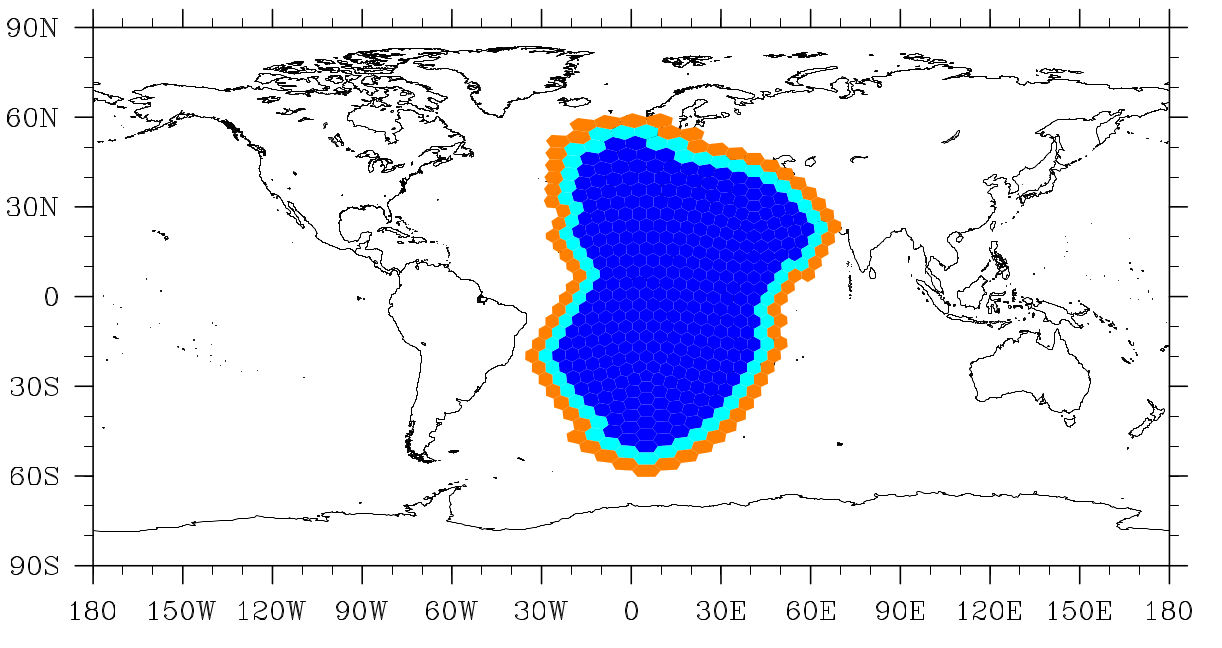
\includegraphics[scale=0.3]{figures/CellHalos.png}
	\caption{The dark blue cells are the block’s owned cells. The light blue are the first halo layer cells and the orange are the second halo layer cells.}
	\label{fig:cell_halos}
\end{figure}

\begin{figure}[htp!]
	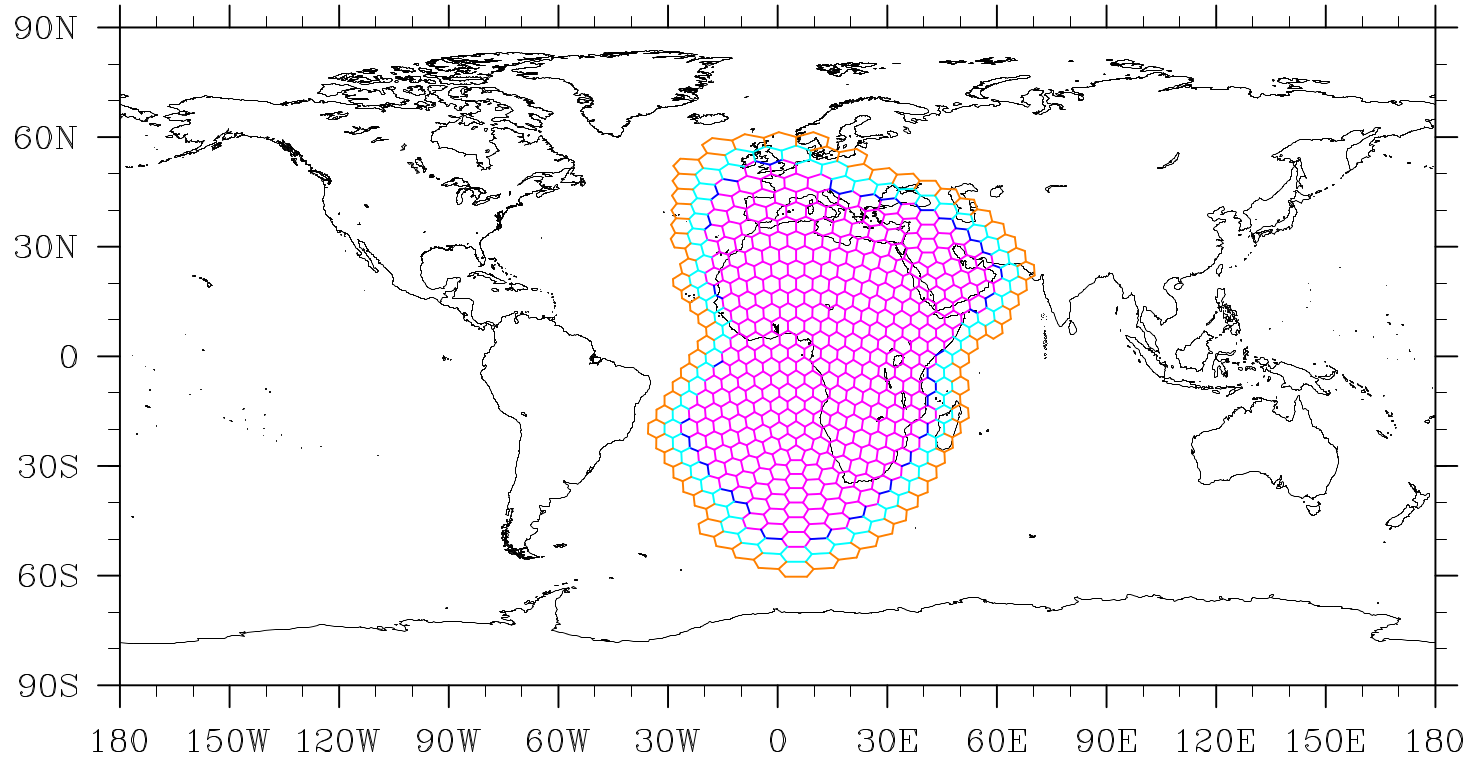
\includegraphics[scale=0.25]{figures/EdgeHalos.png}
	\caption{The pink edges are the block’s owned edges. The dark blue edges on the pink perimeter are the first halo layer edges, the light blue are the second halo layer edges, and the orange are the third halo layer edges.}
	\label{fig:edge_halos}
\end{figure}
\FloatBarrier

Cells make up the primary mesh within MPAS. Halos for cells are described below:
\begin{itemize}
	\item 0-Halo: All "owned" cells;
	\item 1-Halo: All cells that border 0-Halo cells but are not 0-Halo cells;
	\item 2-Halo: All cells that border 1-Halo cells but do not belong to a lesser halo;
	\item 3-Halo: All cells that border 2-Halo cells but do not belong to a lesser halo;
\end{itemize}
Cells can have an arbitrary number of halos, in which case this incremental
definition continues until the last halo layer.

Edges and Vertices have a slightly different definition and always include an additional layer.
\begin{itemize}
	\item 0-Halo: All "owned" edges/vertices;
	\item 1-Halo: All edges/vertices that border 0-Halo cells that are not 0-Halo edges/vertices;
	\item 2-Halo: All edges/vertices that border 1-Halo cells that are not 1-Halo edges/vertices;
	\item 3-Halo: All edges/vertices that border 2-halo cells that are not 2-Halo edges/vertices;
	\item ...
\end{itemize}
As with cells, edges/vertices past the 1 halo use the same definition until the last halo layer.

MPI communication occurs between these halo layers. One block needs to send
some of it's 0-halo to other blocks, and it needs to receive other block's
0-halo elements to put into it's halo layers. This communication occurs through
exchange lists, which are built during initialization. An exchange list
describes MPI sends, MPI receives, and local copies. 

A local copy occurs when two blocks need to communicate and are owned by the
same MPI task. In this case, the exchange lists describes where data can be
found in the owning blocks list, and where it should go in the receiving blocks
list.

A MPI send exchange list describes what processor the communication needs to
occur with. It also describes what elements need to be read from the owning
blocks list, and where those elements should be placed in the sending buffer.

A MPI receive exchange list describes what processor the communication needs to
occur with. It also describes how to unpack data from the buffer into the halo
layers.

Halo exchange routines are provided in src/framework/mpas\_dmpar.F. These halo
exchange routines internally loop over all blocks in the list of blocks,
starting from the block that was passed in. Because of this, a developer should
always pass in the first block's field (i.e. domain \% blocklist \% struct \%
field) to these routines, and should never put a halo exchange within a block
loop. A halo exchange within a block loop will only work properly if there is
only a single block per processor.

A generic interface for halo exchanges of all fields is provided as follows:
\begin{lstlisting}
mpas_dmpar_exch_halo_field(field, haloLayersIn)
\end{lstlisting}
The argument haloLayersIn is optional, and allows specification of which halo
layers should be communicated. This allows the developer more control over
message size.

Currently there is no standard way of implementing OpenMP in MPAS. None of the
shared code has any OpenMP directives in it, but several developers are
investigating the best method of implementing OpenMP in MPAS.

\chapter{Addition of a new core}
Some developers might want to add a new core to the main MPAS repository,
without having a core maintainer defined yet. The steps of adding a new core
are largely the same as adding a new feature. 

The new core is developed in a fork of the relevant repository. After the new
core is ready to be merged into the main repository, a pull request is
submitted. This pull request can be assigned to any other core maintainer, and
should be reviewed by at least two core maintainers.

The other core maintainers will review the core, and ensure it meets the
requirements set forth in the developers guide. After the new core is approved
to be merged onto the developers repository, a core maintainer may be
designated to handle pull requests related to the new core.

\chapter{Copyright Information}
The MPAS framework is distributed under a BSD license. When developing code for
an existing core, it's important to make sure the copyright on the new code
cooperates well with the copyright for the rest of the core.

Under the BSD license a core could be distributed under a different license,
but that license wouldn't change the license applied to the shared framework.

Please discuss any related copyright issues with the relevant core maintainers
for help deciding which license to use on your software.

The text of the BSD license can be see below:

\begin{verbatim}
Copyright (c) 2013,  Los Alamos National Security, LLC (LANS) (LA-CC-13-047)
and the University Corporation for Atmospheric Research (UCAR).

All rights reserved.

LANS is the operator of the Los Alamos National Laboratory under Contract No.
DE-AC52-06NA25396 with the U.S. Department of Energy.  UCAR manages the National
Center for Atmospheric Research under Cooperative Agreement ATM-0753581 with the
National Science Foundation.  The U.S. Government has rights to use, reproduce,
and distribute this software.  NO WARRANTY, EXPRESS OR IMPLIED IS OFFERED BY
LANS, UCAR OR THE GOVERNMENT AND NONE OF THEM ASSUME ANY LIABILITY FOR THE USE
OF THIS SOFTWARE.  If software is modified to produce derivative works, such
modified software should be clearly marked, so as not to confuse it with the
version available from LANS and UCAR.

Additionally, redistribution and use in source and binary forms, with or without
modification, are permitted provided that the following conditions are met:

1) Redistributions of source code must retain the above copyright notice, this
list of conditions and the following disclaimer.

2) Redistributions in binary form must reproduce the above copyright notice,
this list of conditions and the following disclaimer in the documentation and/or
other materials provided with the distribution.

3) None of the names of LANS, UCAR or the names of its contributors, if any, may
be used to endorse or promote products derived from this software without
specific prior written permission.

THIS SOFTWARE IS PROVIDED BY THE COPYRIGHT HOLDERS AND CONTRIBUTORS "AS IS" AND
ANY EXPRESS OR IMPLIED WARRANTIES, INCLUDING, BUT NOT LIMITED TO, THE IMPLIED
WARRANTIES OF MERCHANTABILITY AND FITNESS FOR A PARTICULAR PURPOSE ARE
DISCLAIMED. IN NO EVENT SHALL THE COPYRIGHT HOLDER OR CONTRIBUTORS BE LIABLE FOR
ANY DIRECT, INDIRECT, INCIDENTAL, SPECIAL, EXEMPLARY, OR CONSEQUENTIAL DAMAGES
(INCLUDING, BUT NOT LIMITED TO, PROCUREMENT OF SUBSTITUTE GOODS OR SERVICES;
LOSS OF USE, DATA, OR PROFITS; OR BUSINESS INTERRUPTION) HOWEVER CAUSED AND ON
ANY THEORY OF LIABILITY, WHETHER IN CONTRACT, STRICT LIABILITY, OR TORT
(INCLUDING NEGLIGENCE OR OTHERWISE) ARISING IN ANY WAY OUT OF THE USE OF THIS
SOFTWARE, EVEN IF ADVISED OF THE POSSIBILITY OF SUCH DAMAGE.
\end{verbatim}

\chapter{Core maintainers}
Each core has a list of maintainers. These lists should be relatively short,
and include developers with write access to the main developers repository.
Core maintainers will be responsible for pull requests into their core, and
possibly shared portions of MPAS. 

Current core maintainers are as follows:
\begin{itemize}
	\item Non-Hydrostatic Atmosphere:
		\begin{itemize}
			\item Michael Duda
			\item Bill Skamarock
		\end{itemize}
	\item Ocean
		\begin{itemize}
			\item Doug Jacobsen
			\item Mark Petersen
			\item Todd Ringler
		\end{itemize}
	\item Shallow Water
		\begin{itemize}
			\item All Other Core Maintainers
		\end{itemize}
\end{itemize}

\end{document}
